\documentclass[serif, pdf]{beamer}

%   Theme
\usetheme{Warsaw}

%   Packages
\usepackage{xcolor}
\usepackage{tikz}
\usepackage{multimedia}
\usepackage{lmodern}
\usepackage{scrextend}
\usepackage{subcaption}
\usepackage[normalem]{ulem}
%\usepackage{media9}
%\usepackage{movie15}

%   To keep the spacing of text in tables
\usepackage{makecell}
%   Parameter for the spacing
\setcellgapes{4pt}

\usepackage{caption}
%   Redefines the caption setup of the Figures environment in the beamer class
\captionsetup[figure]{labelformat=empty}
\setbeamerfont{caption}{size=\scriptsize}

%   Colour theme
\usecolortheme{beaver}

%   Metadata
\title[MOD]{Generation And Simulation Of Manufacturable 2D Soft Bodies}
\date{8 May 2020}
\author[Naud\'e Conradie]{Naud\'e Conradie\\{\small Supervisor: Dr MP Venter}}
\institute[]{Department of Mechanical and Mechatronic Engineering, Stellenbosch University}

%   Colour definitions
\definecolor{colour1}{RGB}{96, 34, 59}
\definecolor{colour2}{RGB}{140, 151, 154}
\setbeamercolor{structure}{fg=colour1,bg=colour2}
\setbeamercolor{title}{fg=white,bg=colour2}
\setbeamercolor{author in head/foot}{fg=colour1}

%   Beamer template settings
\setbeamertemplate{itemize item}{\color{black}$\bullet$}
\setbeamertemplate{itemize subitem}{\color{black}$-$}
\setbeamertemplate{caption}{\raggedright\insertcaption\par}

%   Footer settings
\expandafter\def\expandafter\insertshorttitle\expandafter{%
  \insertshorttitle\hfill%
  \hspace{30mm}\insertframenumber\,/\,\inserttotalframenumber}

\beamertemplatenavigationsymbolsempty

\begin{document}

%   Title Slide-------------------------------------------------%

\begin{frame}
  \begin{center}
    \vspace{0.1cm}
    \includegraphics[scale=0.25]{USlogo.pdf}
  \end{center}
  \titlepage
\end{frame}

%   Overview----------------------------------------------------%

\changefontsizes{13pt}
\begin{frame}
    \frametitle{Presentation Overview}
    \begin{itemize}
        \item<1-> Project scope
        \item<2-> Objectives
        \item<3-> Methodology
        \item<4-> Results
    \end{itemize}
\end{frame}

%   Project Scope-----------------------------------------%

\begin{frame}
    \frametitle{Project Scope}
    \begin{itemize}
        \item<1-> Automate the generation and simulation of 2D soft bodies
        \changefontsizes{11pt}
        \begin{itemize}
            \item<2-> Generate 2D bodies built from smaller building blocks with specific deformations
            \item<3-> Non-linear FEM with hyper-elastic material models
            \item<4-> Evaluate the bodies and building blocks according to predefined goals
        \end{itemize}
    \end{itemize}
\end{frame}

%   Objectives-----------------------------------------%

\begin{frame}
    \frametitle{Objectives}
    \begin{itemize}
        \item<1-> Automation for future use and development
        \item<2-> Generation of soft bodies built from generated smaller units
        \item<3-> Selection of best models according to selected metrics
        \item<4-> Accurate modelling of real-world materials
        \item<5-> Computationally efficient manner
        \item<6-> Limitations
        \changefontsizes{11pt}
        \begin{itemize}
            \item<7-> Two dimensions
            \item<8-> Pre-existing material models
        \end{itemize}
    \end{itemize}
\end{frame}

%   Software----------------------------------------------------%

\changefontsizes{13pt}
\begin{frame}
    \frametitle{Software}
    \begin{itemize}
        \item<1-> LS-Dyna
        \changefontsizes{11pt}
        \begin{itemize}
            \item<2-> License expired
        \end{itemize}
        \item<3-> Siemens NX 12
        \changefontsizes{11pt}
        \begin{itemize}
            \item<4-> Unnecessary
        \end{itemize}
        \item<3-> MSC Marc Mentat
        \changefontsizes{11pt}
        \begin{itemize}
            \item<5-> Python
        \end{itemize}
    \end{itemize}
\end{frame}

%   Methodology-----------------------------------------%

\begin{frame}
    \frametitle{Methodology}
    \begin{itemize}
        \item<1-> Generate grid of square elements
        \item<2-> Random internal elements are removed
        \item<3-> Simulation is evaluated
        \item<4-> Accurate modelling of real-world materials
        \item<5-> Computationally efficient manner
        \item<6-> Limitations
        \changefontsizes{11pt}
        \begin{itemize}
            \item<7-> Two dimensions
            \item<8-> Pre-existing material models
        \end{itemize}
    \end{itemize}
\end{frame}

%   Current Objectives------------------------------------------%

\begin{frame}
    \frametitle{Current Objectives (cont.)}
    \begin{itemize}
        \item<1-> Compare commercial software (NX 12, LSDyna, Marc Mentat)
    \end{itemize}
    \begin{center}
        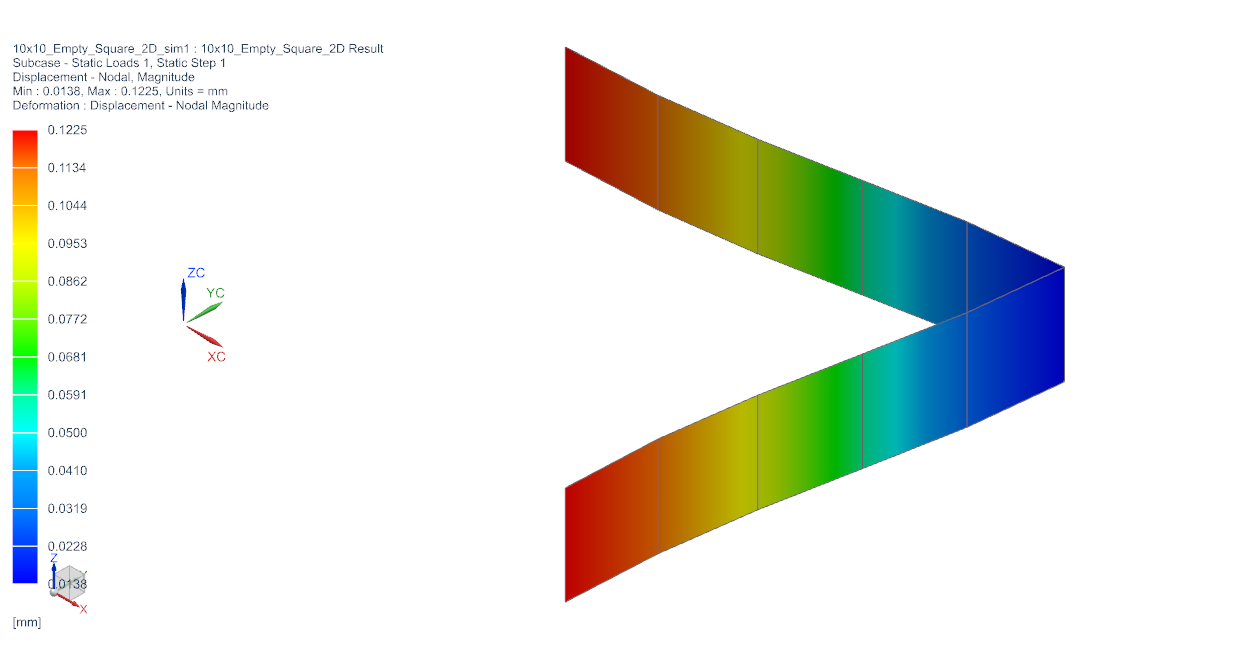
\includegraphics[width=0.35\linewidth]{10x10_Empty_Square_2D_Deformation.png}
    \end{center}
    \begin{itemize}
        \item<2-> Implementation with code from N Kim and open source software
    \end{itemize}
\end{frame}

%   Current Objectives------------------------------------------%

\begin{frame}
    \frametitle{Current Objectives (cont.)}
    \begin{itemize}
        \item<1-> Compare modeled behaviour to actual behaviour
        \changefontsizes{11pt}
        \begin{itemize}
            \item<2-> Produce square
            \item<2-> Place between two transparent plates
            \item<2-> Apply pressure
            \item<2-> Observe and compare
        \end{itemize}
        \item<3-> Determine which approach
        \changefontsizes{11pt}
        \begin{itemize}
            \item<4-> Commercial vs. open-source vs. own code
            \item<5-> All have pros and cons
        \end{itemize}
    \end{itemize}
\end{frame}

%   Further Objectives------------------------------------------%

\begin{frame}
    \frametitle{Further Objectives}
    \begin{itemize}
        \item<1-> Define unit cell behaviour
    \end{itemize}
    \begin{figure}
        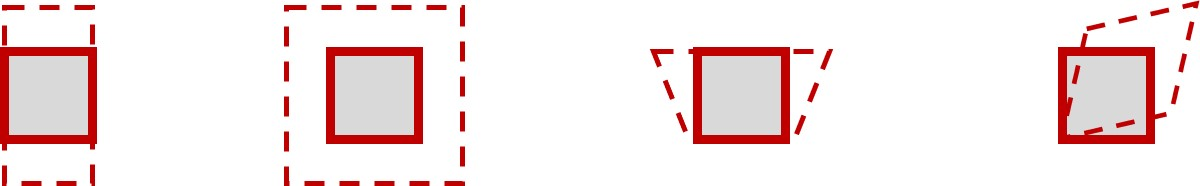
\includegraphics[height = 1cm]{Unit_Cell_Deformation.jpg}<1->
    \end{figure}
    \begin{itemize}
        \item<2-> Define recursive rules
        \item<3-> Set up genetic algorithm
        \item<4-> Combine all components
    \end{itemize}
\end{frame}

%   Questions---------------------------------------------------%

\begin{frame}
    \begin{center}
        \huge Questions?
    \end{center}
\end{frame}

\end{document}
